% !Mode:: "TeX:UTF-8"
%!TEX program  = xelatex

\documentclass[bwprint]{gmcmthesis}
\usepackage[framemethod=TikZ]{mdframed}
\usepackage{longtable}
\usepackage{lineno,hyperref}
\usepackage{amsmath}
\usepackage{float}
\usepackage{graphicx}
\usepackage{subfigure}
\usepackage{caption}
\title{全国研究生数学建模竞赛论文标题}
\baominghao{4321} %参赛队号
\schoolname{XX大学}%学校名称
\membera{小米} %队员A
\memberb{向左} %队员B
\memberc{哈哈} %队员C
\begin{document}

 %生成标题
 \maketitle

 %填写摘要
\begin{abstract}
本模板是为全国研究生数学建模竞赛编写的 \LaTeX{} 模板, 旨在让大家专注于
论文的内容写作, 而不用花费过多精力在格式的定制和调整上. 本手册是相应的参考, 其
中提供了一些环境和命令可以让模板的使用更为方便. 同时需要注意, 使用者需要有一
定的 \LaTeX{} 的使用经验, 至少要会使用 ctex 宏包的一些功能, 比如调节字距或修改字体
大小等等.


 \begin{mdframed} [%
	roundcorner=5pt,
	linecolor=gray!50,
	outerlinewidth=0.5pt,
	middlelinewidth=0.3pt, backgroundcolor=gray!2,
innertopmargin=\topskip, frametitle={2020年格式变化说明},
frametitlefont= \bfseries,frametitlerule=true,frametitlealignment =\raggedright\noindent,
frametitlerulewidth=.5pt, frametitlebackgroundcolor=gray!2,]
今年的格式变化如下:
\begin{enumerate}
\item 论文第一页为标识替换。

\end{enumerate}

\end{mdframed}



欢迎大家到QQ群里沟通交流:91940767/478023327/640633524。我们也开通了问答区交流 \LaTeX{}技术:\url{https://wenda.latexstudio.net},欢迎大家前来交流。


\uwave{关注我们的微信公众号}:

\centerline{
\includegraphics[width=11cm]{gongzhonghao}}


\keywords{模板\quad  \LaTeX{}\quad   数学建模}
\end{abstract}

\pagestyle{plain}

%目录 不推荐加
%\tableofcontents

\section{问题重述}

\subsection{引言}

近年来,基于文本形式的在线旅游与用户生成内容愈发成为人们获取旅游信息进行攻略查询的重要信息来源。在这些信息中,有许多内容蕴含丰富的旅游相关信息,比如各文旅实体可能之间存在某种内在联系能够通过一定手段被挖掘出来,进而能够用作数据分析、营销产品设计及推荐系统等业务。因此,从众多文本数据中筛选出与文旅主题相关的信息,进而运用知识图谱手段挖掘文旅实体之间内在联系具有重要意义。

\subsection{问题的提出}

\begin{itemize}
	\item 问题一:针对附件中的微信公众号新闻子表,根据其中公众号推文与文旅的相关度进行分类。与文旅相关的高频主题词可能包括:旅游,活动,交通,酒店,景区,假期,游客,农家乐等。
 
	\item 问题二:根据表格中对景区、酒店等旅游产品的实例和信息,将提取出的旅游产品进行提取。随后构建模型从多维度对产品的热度进行评价。
 
	\item 问题三:根据表格中的OTA、UGC数据,对旅游产品进行关联度分析,找出以景区、酒店、餐饮为核心的强关联模式。并在此基础上进行可视化分析。
 
	\item 问题四:基于历史数据,分析疫情前后旅游产品变化。
\end{itemize}


% \section{模型的假设}

% \begin{itemize}
% \item 忽略实际加工误差对设计的影响;
% \item 木条与圆桌面之间的交接处缝隙较小,可忽略;
% \item 钢筋强度足够大,不弯曲;
% \item 假设地面平整。
% \end{itemize}

% \section{符号说明}

% \begin{tabular}{cc}
%  \hline
%  \makebox[0.4\textwidth][c]{符号}	&  \makebox[0.5\textwidth][c]{意义} \\ \hline
%  D	    & 木条宽度(cm) \\ \hline
%  L	    & 木板长度(cm)  \\ \hline
%  W	    & 木板宽度(cm)  \\ \hline
%  N	    & 第n根木条  \\ \hline
%  T	    & 木条根数  \\ \hline
%  H	    & 桌子高度(cm)  \\ \hline
%  R	    & 桌子半径(cm)  \\ \hline
%  R	    & 桌子直径(cm)  \\ \hline
% \end{tabular}

\section{问题分析}

\subsection{问题一分析}
利用附件中提供的公众号推文和游记攻略,本文需要构建适当模型根据其与文旅主题的相关性进行样本的有效划分。

首先,公众号推文包含标题、发表时间和正文信息。经过初步观察,推文标题和正文中都包含相与文旅相关的主题词,但其中有些正文内容收到其本身是广告或图片的形式,导致其内容体现在正文文本上与文旅主题相关程度不高。针对这类数据的预处理直接影响后续文本分类模型的好坏。

其次,游记攻略相关信息包括城市、游记标题、发布时间、出发时间、出行天数、人物、费用及正文。经过初步观察,游记攻略的标题和正文蕴含着丰富文本信息,但其中同样存在一些不相关的内容需要甄别,这也对后续的分类模型带来一定的挑战。


\subsection{问题二分析}
对旅游产品进行特征工程,最直观的为旅游产品被提及的次数。其他可能的思路包括旅游产品评价的高频词提取,评论情感倾向识别。


% \begin{figure}[!h]
% \centering
% 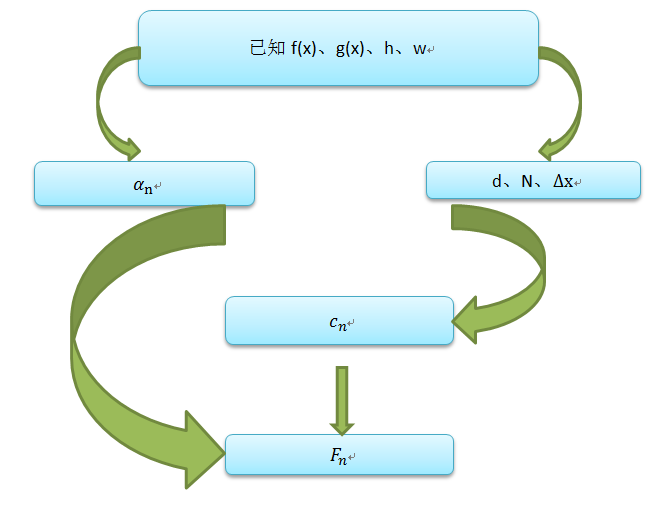
\includegraphics[width=.7\textwidth]{1.png}
% \caption{问题三流程图}
% \end{figure}

\subsection{问题三分析}
关联度构建可以考虑由公众号新闻和攻略出发进行挖掘。

\subsection{问题一建模与求解}

\subsubsection{数据预处理}

根据前文分析,公众号推文和游记的标题与正文都一定程度包含与文旅相关的内容,故本文将标题与正文进行合并,用于后续的分析。对于已经获得的文本,本文对其进行数据清理,将其中的数字、字母、特殊字符、换行符和空格等进行删除,并随后对字段进行分词处理。

\subsubsection{模型构建与求解}

针对已有的文本,本文考虑构建LDA(Latent Dirichlet Allocation)主题模型实现文章与文旅相关性的划分。LDA模型利用了贝叶斯的思想,将每个文本和每个主题词的先验分布均视为狄利克雷(Dirichlet)分布,其中文本词向量一致,目标是求语料库的分布。
\begin{gather}
	\theta_d \sim Dirichlet(\alpha) \\
	\beta_k \sim Dirichlet(\eta)
\end{gather}


其中随机变量$\theta_d$与$\beta_k$分别代表第$d$条文本和第$k$个主题词,$\alpha$和$\eta$分别代表分布的超参数向量,维度分别为$K$和$V$。对于第$d$条文本中的第$n$个词,根据多项分布可以得到其主题编号$z_{dn} \sim multi(\theta_d)$和词分布$w_{dn} \sim multi(\beta_{z_{dn}})$。则$(\alpha \rightarrow \theta_d \rightarrow z_d)$组成了Dirichlet-multi共轭分布。故能够得到$\theta_d$的后验分布$Dirichlet(\theta_d|\alpha + n_d)$,同样可以得到$\beta_k$的后验分布$Dirichlet(\beta_k|\eta + n_k)$。LDA模型的任务便是需要得到收敛的主题词$\beta$分布。至于LDA模型的求解,本文选用基于变分推断的EM算法。

首先本文给LDA主题模型设定了一系列主题词总共38个,包括:“旅游、活动、节庆、特产、交通、酒店、景区、景点、文创、文化、乡村旅游、民宿、假日、假期、游客、采摘、赏花、春游、踏青、康养、公园、滨海游、度假、农家乐、剧本杀、旅行、徒步、工业旅游、线路、自驾游、 团队游、攻略、游记、包车、玻璃栈道、游艇、高尔夫、温泉”。随后,运用LDA主题模型得到每条文本分属$K$个分类的概率,并统计了每个类中的单词的出现频率,并提取其中最常出现的$D$个词汇, 上述$D$,$K$为模型超参数。

对LDA主题模型分得的$K$个类别,本文将其中每类的高频词汇提出,分别将每类对应的高频词汇与文旅相关主题词进行匹配,匹配度达到一定阈值$\gamma$则认定该类属于与文旅主题相关,否则为不相关,值得一提的是阈值$\gamma$在本文中也为超参数。此外本文通过pyLDAvid和pyLDAvis对主题进行可视化。



对于公众号推文,本文发现,在超参数$K=6$,$\gamma=0$的时候,分类的效果较为理想,经过初步可视化,以其中四个分类的高频词为例,如下图所示:


\begin{figure}[H]
	\centering
	\begin{minipage}{0.49\linewidth}
		\centering
		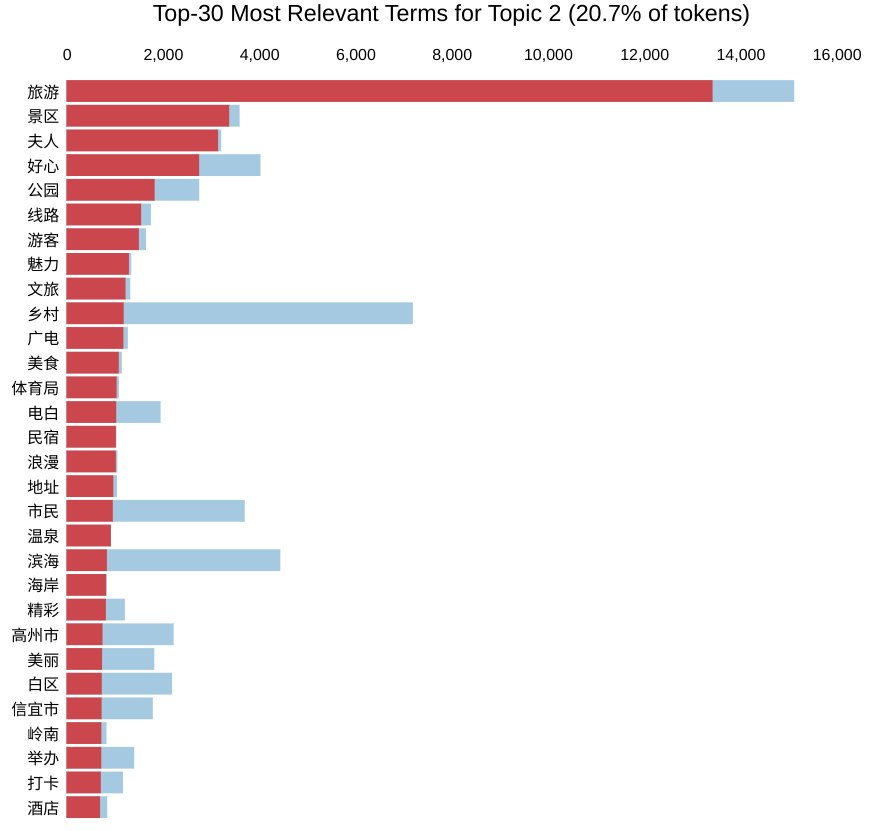
\includegraphics[width=0.9\linewidth]{figures/news1.png}
		\caption{分类2}
		\label{news1}%文中引用该图片代号
	\end{minipage}
	\begin{minipage}{0.49\linewidth}
		\centering
		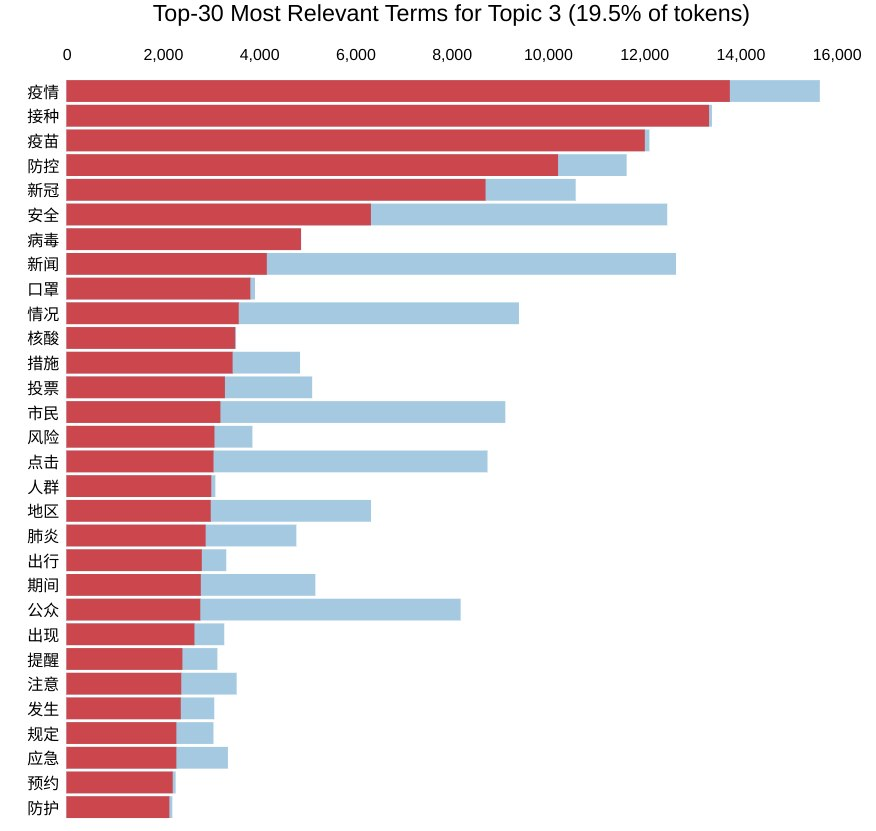
\includegraphics[width=0.9\linewidth]{figures/news2.png}
		\caption{分类3}
		\label{news2}%文中引用该图片代号
	\end{minipage}
	%\qquad
	%让图片换行,
	
	\begin{minipage}{0.49\linewidth}
		\centering
		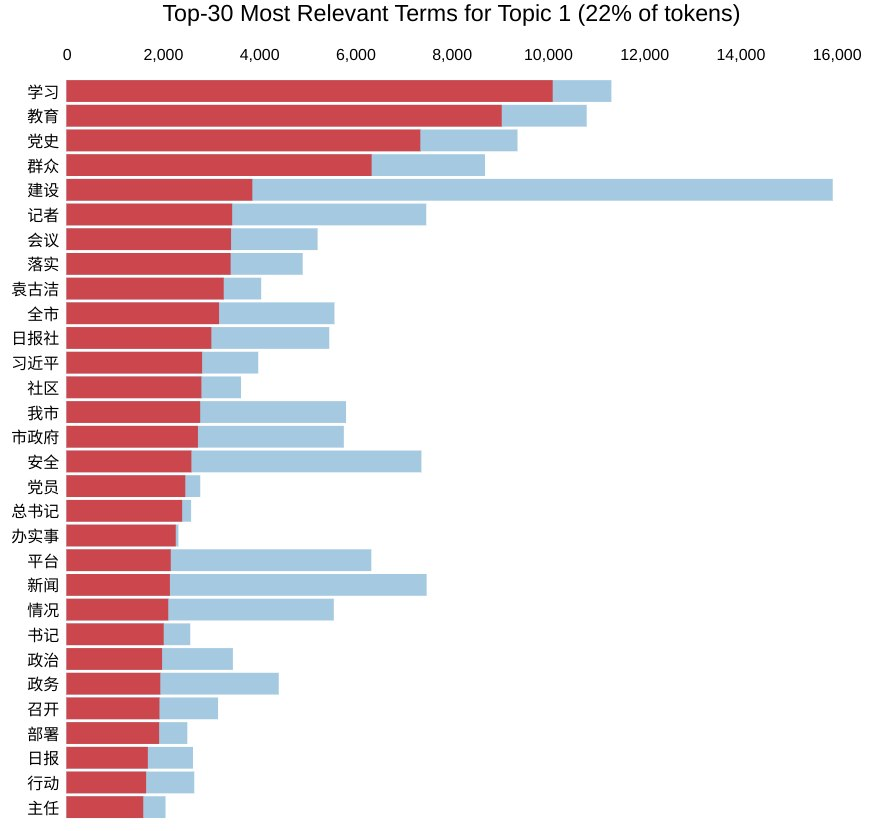
\includegraphics[width=0.9\linewidth]{figures/news3.png}
		\caption{分类1}
		\label{news3}%文中引用该图片代号
	\end{minipage}
	\begin{minipage}{0.49\linewidth}
		\centering
		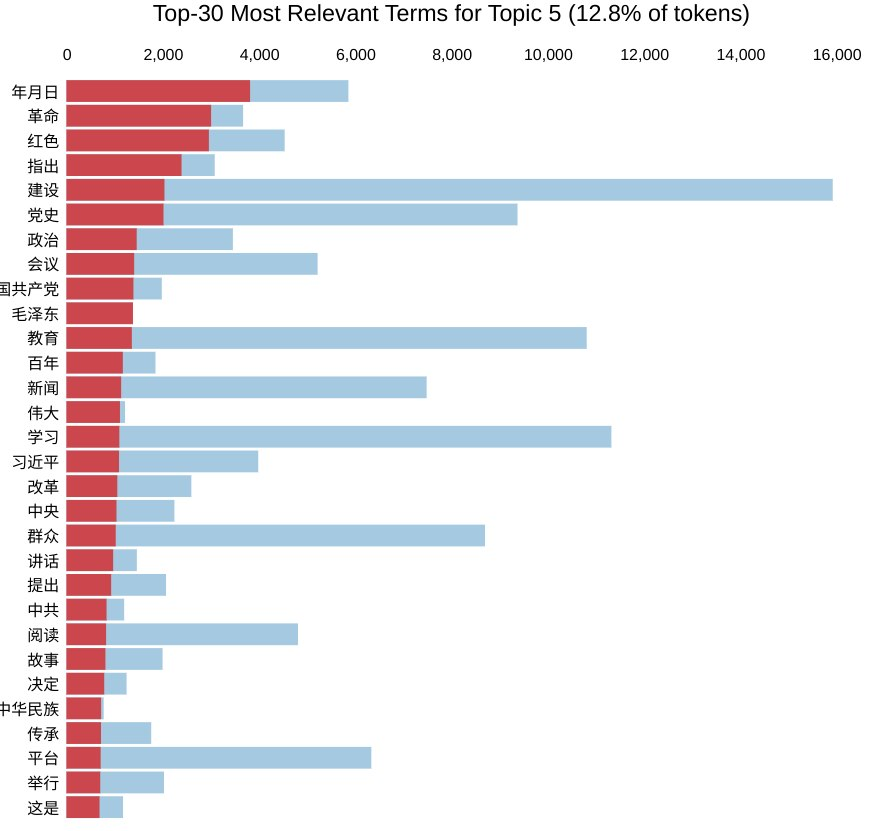
\includegraphics[width=0.9\linewidth]{figures/news4.png}
		\caption{分类5}
		\label{news4}%文中引用该图片代号
	\end{minipage}
\end{figure}

经过初步观察,基于LDA的建模是有效的,文旅相关的文本被提取了出来,其余的分类包括新冠疫情或党建主题。

对于旅游攻略,本文发现,在超参数$K=5$,$\gamma=0$的时候,分类的效果较为理想,经过初步可视化,以其中两个分类的高频词为例,如下图所示:

\begin{figure}[H]
    \centering
    \subfigure[分类1]{
        \label{travel1}
        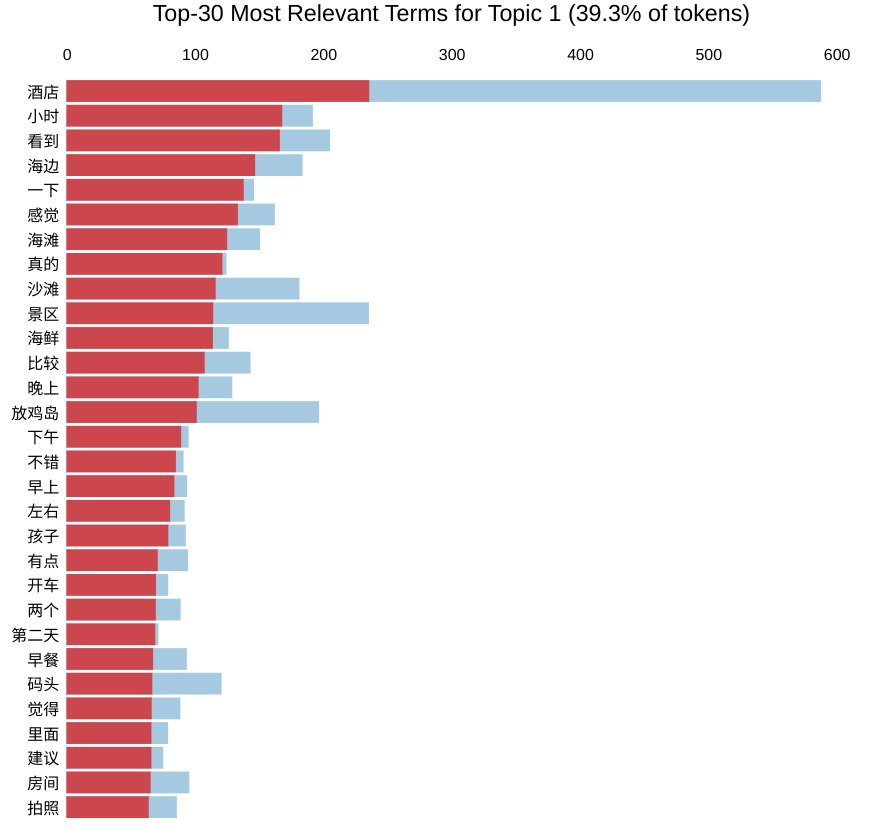
\includegraphics[width=0.45\textwidth]{figures/travel1.png}
    }
    \hspace{0in}
    \subfigure[分类2]{
        \label{travel2}
        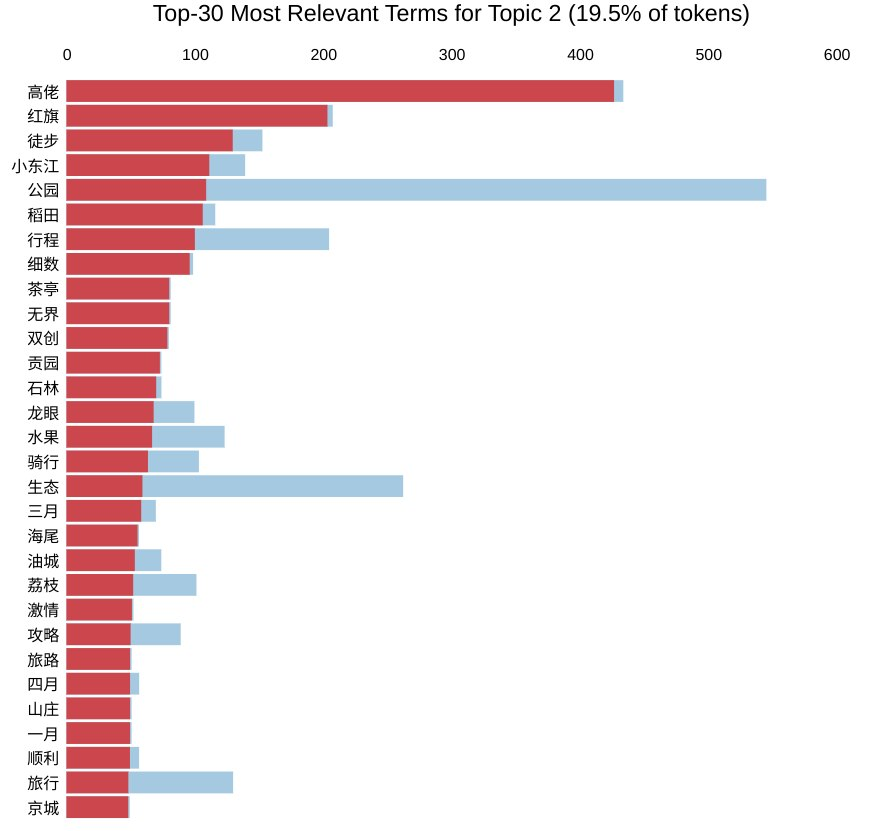
\includegraphics[width=0.45\textwidth]{figures/travel2.png}
    }
    \caption{基于LDA模型的旅游攻略词频分析}
    \label{travel_cipin}
\end{figure}

通过图\ref{travel_cipin}能够看出,LDA主题模型的分类对于旅游攻略文本同样是有效的,文旅相关的文本与党建等无关主题的文本被有效提取了出来。

下表给出了微信公众号推文和游记攻略与文旅主题相关性的判断:

%参考文献   手工录入
%\begin{thebibliography}{9}%宽度9
% \bibitem{bib:one} ....
% \bibitem{bib:two} ....
%\end{thebibliography}

%采用bibtex方案
\cite{wright_latex3_2009}

\bibliographystyle{gmcm}
\bibliography{example}


\newpage
%附录
\appendix
%\setcounter{page}{1} %如果需要可以自行重置页码。
\section{我的 MATLAB 源程序}
\begin{lstlisting}[language=Matlab]%设置不同语言即可。
kk=2;[mdd,ndd]=size(dd);
while ~isempty(V)
[tmpd,j]=min(W(i,V));tmpj=V(j);
for k=2:ndd
[tmp1,jj]=min(dd(1,k)+W(dd(2,k),V));
tmp2=V(jj);tt(k-1,:)=[tmp1,tmp2,jj];
end
tmp=[tmpd,tmpj,j;tt];[tmp3,tmp4]=min(tmp(:,1));
if tmp3==tmpd, ss(1:2,kk)=[i;tmp(tmp4,2)];
else,tmp5=find(ss(:,tmp4)~=0);tmp6=length(tmp5);
if dd(2,tmp4)==ss(tmp6,tmp4)
ss(1:tmp6+1,kk)=[ss(tmp5,tmp4);tmp(tmp4,2)];
else, ss(1:3,kk)=[i;dd(2,tmp4);tmp(tmp4,2)];
end;end
dd=[dd,[tmp3;tmp(tmp4,2)]];V(tmp(tmp4,3))=[];
[mdd,ndd]=size(dd);kk=kk+1;
end; S=ss; D=dd(1,:);


 \end{lstlisting}


\end{document} 